\documentclass[aspectratio=169]{beamer}
\usetheme{Madrid}
\usecolortheme{default}

% Packages
\usepackage{amsmath}
\usepackage{amssymb}
\usepackage{listings}
\usepackage{xcolor}
\usepackage{tikz}
\usepackage{algorithm}
\usepackage{algorithmic}
\usepackage{booktabs}

% TikZ libraries
\usetikzlibrary{shapes,arrows,positioning,fit,calc}

% Code listing style
\lstset{
  basicstyle=\ttfamily\tiny,
  keywordstyle=\color{blue},
  commentstyle=\color{green!60!black},
  stringstyle=\color{red},
  breaklines=true,
  frame=single
}

% Title information
\title[CasADi-Based MPC for Social Navigation]{CasADi-Based Model Predictive Control for Socially-Aware Robot Navigation}
\subtitle{Optimization Pipeline and VLM Integration}
\author{Social MPC Navigation Stack}
\institute{TIAGo Mobile Robot - ROS 2 Humble}
\date{\today}

\begin{document}

% ============================================================
% TITLE SLIDE
% ============================================================
\begin{frame}
  \titlepage
\end{frame}

% ============================================================
% TABLE OF CONTENTS
% ============================================================
\begin{frame}{Outline}
  \tableofcontents
\end{frame}

% ============================================================
% SECTION 1: OVERVIEW
% ============================================================
\section{System Overview}

\begin{frame}{System Overview}
  \begin{columns}[T]
    \begin{column}{0.5\textwidth}
      \textbf{Navigation Stack Components:}
      \begin{enumerate}
        \item \textcolor{blue}{Global Planner}: A* path planning
        \item \textcolor{blue}{Ground-Truth Localization}: Perfect pose estimation
        \item \textcolor{blue}{People Adapter}: Crowd state tracking
        \item \textcolor{blue}{VLM Integration}: Scene understanding
        \item \textcolor{blue}{VLM Translator}: Semantic $\rightarrow$ numerical
        \item \textcolor{red}{\textbf{CasADi MPC Controller}}: Local trajectory optimization
      \end{enumerate}
    \end{column}
    \begin{column}{0.5\textwidth}
      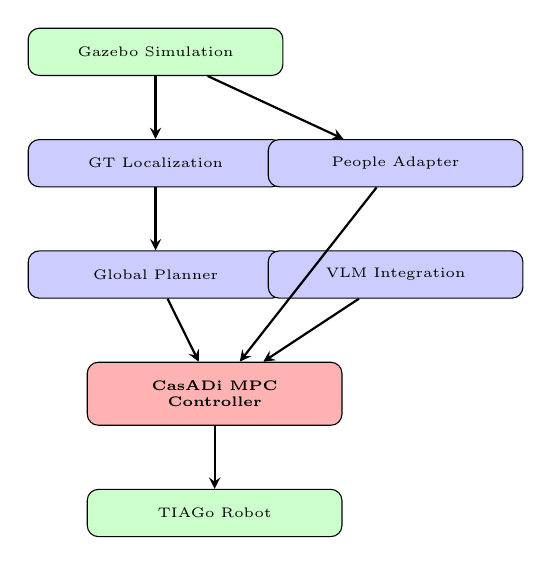
\begin{tikzpicture}[
        node distance=0.8cm,
        block/.style={rectangle, draw, fill=blue!20, text width=3cm, text centered, rounded corners, minimum height=0.6cm, font=\tiny},
        sensor/.style={rectangle, draw, fill=green!20, text width=3cm, text centered, rounded corners, minimum height=0.6cm, font=\tiny},
        controller/.style={rectangle, draw, fill=red!30, text width=3cm, text centered, rounded corners, minimum height=0.8cm, font=\tiny\bfseries},
        arrow/.style={->, >=stealth, thick}
      ]
        % Perception layer
        \node[sensor] (gazebo) {Gazebo Simulation};
        \node[block, below=of gazebo] (loc) {GT Localization};
        \node[block, right=of loc, xshift=-1cm] (people) {People Adapter};

        % Planning layer
        \node[block, below=of loc] (planner) {Global Planner};
        \node[block, right=of planner, xshift=-1cm] (vlm) {VLM Integration};

        % Control layer
        \node[controller, below=of planner, xshift=0.75cm] (mpc) {CasADi MPC\\Controller};

        % Robot
        \node[sensor, below=of mpc] (robot) {TIAGo Robot};

        % Arrows
        \draw[arrow] (gazebo) -- (loc);
        \draw[arrow] (gazebo) -- (people);
        \draw[arrow] (loc) -- (planner);
        \draw[arrow] (planner) -- (mpc);
        \draw[arrow] (people) -- (mpc);
        \draw[arrow] (vlm) -- (mpc);
        \draw[arrow] (mpc) -- (robot);
      \end{tikzpicture}
    \end{column}
  \end{columns}

  \vspace{0.5cm}
  \begin{block}{Key Features}
    Real-time optimization-based control with social awareness, obstacle avoidance, and VLM-guided semantic constraints
  \end{block}
\end{frame}

% ============================================================
% SECTION 2: PROBLEM FORMULATION
% ============================================================
\section{Problem Formulation}

\begin{frame}{Navigation Challenge}
  \begin{columns}[T]
    \begin{column}{0.5\textwidth}
      \textbf{Objectives:}
      \begin{itemize}
        \item \textcolor{green}{Goal reaching}: Navigate to target position
        \item \textcolor{orange}{Social navigation}: Respect personal space
        \item \textcolor{red}{Collision avoidance}: Safe obstacle clearance
        \item \textcolor{blue}{Smooth motion}: Comfortable trajectories
      \end{itemize}

      \vspace{0.3cm}
      \textbf{Constraints:}
      \begin{itemize}
        \item Velocity limits: $v \in [0, v_{\max}]$, $\omega \in [-\omega_{\max}, \omega_{\max}]$
        \item Nonholonomic dynamics (unicycle model)
        \item Real-time requirements ($<$ 50ms per cycle)
        \item Dynamic environments (moving people)
      \end{itemize}
    \end{column}

    \begin{column}{0.5\textwidth}
      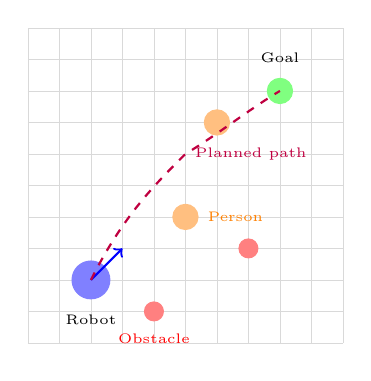
\begin{tikzpicture}[scale=0.8]
        % Grid
        \draw[step=0.5cm, gray!30, very thin] (0,0) grid (5,5);

        % Robot
        \filldraw[blue!50] (1,1) circle (0.3cm);
        \draw[->, thick, blue] (1,1) -- (1.5,1.5);
        \node[below] at (1,0.6) {\tiny Robot};

        % Goal
        \filldraw[green!50] (4,4) circle (0.2cm);
        \node[above] at (4,4.3) {\tiny Goal};

        % People
        \filldraw[orange!50] (2.5,2) circle (0.2cm);
        \filldraw[orange!50] (3,3.5) circle (0.2cm);
        \node[right, orange] at (2.7,2) {\tiny Person};

        % Obstacles
        \filldraw[red!50] (2,0.5) circle (0.15cm);
        \filldraw[red!50] (3.5,1.5) circle (0.15cm);
        \node[below, red] at (2,0.3) {\tiny Obstacle};

        % Path (rough sketch)
        \draw[dashed, thick, purple] (1,1) .. controls (1.5,2) and (2,2.5) .. (2.5,3) .. controls (3,3.3) and (3.5,3.7) .. (4,4);
        \node[purple, right] at (2.5,3) {\tiny Planned path};
      \end{tikzpicture}
    \end{column}
  \end{columns}

  \vspace{0.3cm}
  \begin{alertblock}{Challenge}
    Balance multiple conflicting objectives in real-time within a constrained optimization framework
  \end{alertblock}
\end{frame}

\begin{frame}{Robot Dynamics: Unicycle Model}
  \begin{columns}[T]
    \begin{column}{0.55\textwidth}
      \textbf{State Variables:}
      \begin{align*}
        \mathbf{x}_t &= [x_t, y_t, \theta_t]^T \\
        \mathbf{u}_t &= [v_t, \omega_t]^T
      \end{align*}

      \vspace{0.2cm}
      \textbf{Discrete-Time Dynamics:}
      \begin{align*}
        x_{t+1} &= x_t + v_t \cos(\theta_t) \cdot \Delta t \\
        y_{t+1} &= y_t + v_t \sin(\theta_t) \cdot \Delta t \\
        \theta_{t+1} &= \theta_t + \omega_t \cdot \Delta t
      \end{align*}

      \vspace{0.2cm}
      Where:
      \begin{itemize}
        \item $(x_t, y_t)$: Robot position [m]
        \item $\theta_t$: Robot heading [rad]
        \item $v_t$: Linear velocity [m/s]
        \item $\omega_t$: Angular velocity [rad/s]
        \item $\Delta t = 0.2$s: Discretization timestep
      \end{itemize}
    \end{column}

    \begin{column}{0.45\textwidth}
      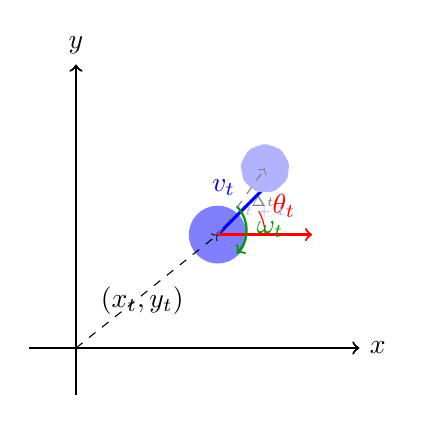
\begin{tikzpicture}[scale=1.2]
        % Coordinate system
        \draw[->, thick] (-0.5,0) -- (3,0) node[right] {$x$};
        \draw[->, thick] (0,-0.5) -- (0,3) node[above] {$y$};

        % Robot at position
        \filldraw[blue!50] (1.5,1.2) circle (0.3cm);
        \draw[->, very thick, blue] (1.5,1.2) -- (2.1,1.8) node[midway, above left] {$v_t$};

        % Heading angle
        \draw[->, thick, red] (1.5,1.2) -- (2.5,1.2);
        \draw[red] (2,1.2) arc (0:30:0.5cm);
        \node[red] at (2.2,1.5) {$\theta_t$};

        % Angular velocity
        \draw[->, thick, green!60!black] (1.7,1.5) to[bend left=45] node[right] {$\omega_t$} (1.7,1.0);

        % Position vector
        \draw[->, dashed] (0,0) -- (1.5,1.2);
        \node at (0.7,0.5) {$(x_t, y_t)$};

        % Next position (prediction)
        \filldraw[blue!30, dashed] (2.0,1.9) circle (0.25cm);
        \draw[->, dashed, gray] (1.5,1.2) -- (2.0,1.9) node[midway, right] {\tiny $\Delta t$};
        \node[below, blue!30] at (2.0,1.6) {\tiny $t+1$};
      \end{tikzpicture}
    \end{column}
  \end{columns}

  \vspace{0.3cm}
  \begin{block}{Nonholonomic Constraint}
    Robot can only move in the direction it's facing (like a car) - cannot move sideways
  \end{block}
\end{frame}

% ============================================================
% SECTION 3: CASADI MPC FORMULATION
% ============================================================
\section{CasADi MPC Formulation}

\begin{frame}{Model Predictive Control (MPC) Concept}
  \begin{columns}[T]
    \begin{column}{0.5\textwidth}
      \textbf{MPC Strategy:}
      \begin{enumerate}
        \item Predict future states over horizon $N$
        \item Optimize control sequence $\mathbf{u}_{0:N-1}$
        \item Apply only first control $\mathbf{u}_0$
        \item Repeat at next timestep (receding horizon)
      \end{enumerate}

      \vspace{0.3cm}
      \textbf{Parameters:}
      \begin{itemize}
        \item Horizon: $N = 15$ steps
        \item Timestep: $\Delta t = 0.2$s
        \item Lookahead: $3.0$s into future
        \item Control rate: $10$ Hz
      \end{itemize}

      \vspace{0.3cm}
      \textbf{Decision Variables:}
      \begin{itemize}
        \item $\mathbf{v} = [v_0, v_1, \ldots, v_{N-1}]$: Linear velocities
        \item $\boldsymbol{\omega} = [\omega_0, \omega_1, \ldots, \omega_{N-1}]$: Angular velocities
        \item Total: $2N = 30$ variables
      \end{itemize}
    \end{column}

    \begin{column}{0.5\textwidth}
      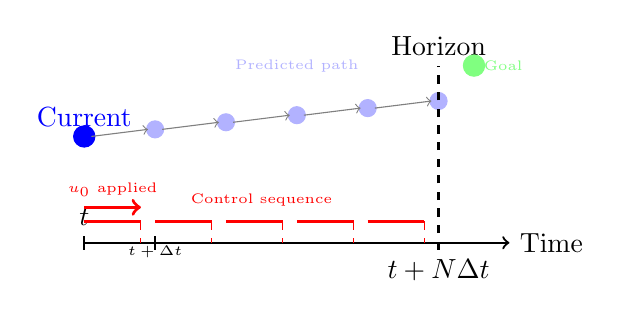
\begin{tikzpicture}[scale=0.9]
        % Time axis
        \draw[->, thick] (0,0) -- (6,0) node[right] {Time};

        % Current time marker
        \draw[thick] (0,-0.1) -- (0,0.1) node[above] {$t$};
        \filldraw[blue] (0,1.5) circle (0.15cm) node[above] {Current};

        % Predicted trajectory
        \foreach \i in {1,...,5} {
          \pgfmathsetmacro{\x}{\i}
          \pgfmathsetmacro{\xstart}{\i-0.9}
          \pgfmathsetmacro{\xend}{\i-0.1}
          \pgfmathsetmacro{\ypos}{1.5+0.1*\i}
          \pgfmathsetmacro{\yposprev}{1.5+0.1*(\i-1)}
          \filldraw[blue!30] (\x,\ypos) circle (0.12cm);
          \draw[->, gray] (\xstart,\yposprev) -- (\xend,\ypos);
        }

        % Horizon marker
        \draw[thick, dashed] (5,-0.1) -- (5,2.5);
        \node[below] at (5,-0.1) {$t+N\Delta t$};
        \node[above] at (5,2.5) {Horizon};

        % Control sequence
        \foreach \i in {0,...,4} {
          \pgfmathsetmacro{\x}{\i}
          \pgfmathsetmacro{\xend}{\i+0.8}
          \draw[red, very thick] (\x,0.3) -- (\xend,0.3);
          \draw[red, dashed] (\xend,0.3) -- (\xend,0);
        }
        \draw[->, red, very thick] (0,0.5) -- (0.8,0.5) node[midway, above] {\tiny $u_0$ applied};

        % Next timestep
        \draw[thick] (1,-0.1) -- (1,0.1) node[below] {\tiny $t+\Delta t$};

        % Goal
        \filldraw[green!50] (5.5,2.5) circle (0.15cm) node[right] {\tiny Goal};

        % Label
        \node[blue!30] at (3,2.5) {\tiny Predicted path};
        \node[red] at (2.5,0.6) {\tiny Control sequence};
      \end{tikzpicture}

      \vspace{0.3cm}
      \begin{alertblock}{Receding Horizon}
        Optimization is resolved at each timestep with updated measurements - adaptive to dynamic environments
      \end{alertblock}
    \end{column}
  \end{columns}
\end{frame}

\begin{frame}{Optimization Problem Structure}
  \begin{block}{Standard MPC Formulation}
    \begin{align*}
      \min_{\mathbf{v}, \boldsymbol{\omega}} \quad & J(\mathbf{x}_{0:N}, \mathbf{u}_{0:N-1}) \\
      \text{subject to} \quad & \mathbf{x}_{k+1} = f(\mathbf{x}_k, \mathbf{u}_k), \quad k = 0, \ldots, N-1 \\
      & 0 \leq v_k \leq v_{\max}, \quad k = 0, \ldots, N-1 \\
      & -\omega_{\max} \leq \omega_k \leq \omega_{\max}, \quad k = 0, \ldots, N-1 \\
      & \mathbf{x}_0 = \mathbf{x}_{\text{current}}
    \end{align*}
  \end{block}

  \vspace{0.3cm}

  \textbf{Why CasADi?}
  \begin{itemize}
    \item \textbf{Automatic Differentiation}: Exact gradients for optimization
    \item \textbf{Symbolic Framework}: Build problem once, update parameters
    \item \textbf{Efficient Solvers}: IPOPT (interior-point) with warm-starting
    \item \textbf{Flexibility}: Easy to modify cost function and constraints
    \item \textbf{Performance}: Compiled C++ code generation possible
  \end{itemize}
\end{frame}

\begin{frame}[fragile]{CasADi Implementation: Problem Setup}
  \begin{columns}[T]
    \begin{column}{0.58\textwidth}
      \begin{lstlisting}[language=C++, caption=setupCasADiProblem() - Build Once]
// Create optimization problem (ONCE at initialization)
opti_ = Opti();

// Decision variables (2*N)
v_var_ = opti_.variable(N_);  // Linear velocities
w_var_ = opti_.variable(N_);  // Angular velocities

// Parameters (updated each iteration)
x0_param_ = opti_.parameter();      // Initial state
y0_param_ = opti_.parameter();
yaw0_param_ = opti_.parameter();

goal_x_param_ = opti_.parameter();  // Goal
goal_y_param_ = opti_.parameter();

v_max_param_ = opti_.parameter();   // From social contract

// Fixed-size arrays for dynamic obstacles
max_obstacles_ = 5;  // Capacity
max_people_ = 5;

obstacles_x_param_ = opti_.parameter(max_obstacles_);
obstacles_y_param_ = opti_.parameter(max_obstacles_);
people_x_param_ = opti_.parameter(max_people_);
people_y_param_ = opti_.parameter(max_people_);
      \end{lstlisting}
    \end{column}

    \begin{column}{0.42\textwidth}
      \textbf{Key Insight:}
      \begin{itemize}
        \item Problem structure built \textcolor{red}{once}
        \item Only \textcolor{blue}{parameter values} updated each iteration
        \item Avoids symbolic recompilation overhead
      \end{itemize}

      \vspace{0.3cm}
      \textbf{Fixed-Size Parameters:}
      \begin{itemize}
        \item Preallocate max capacity
        \item Inactive elements set to $(10^6, 10^6)$
        \item Distance $\rightarrow \infty$, cost $\rightarrow 0$
        \item Maintains constant problem structure
      \end{itemize}

      \vspace{0.3cm}
      \begin{alertblock}{Performance}
        This design enables \textbf{warm-starting} and \textbf{10-50x speedup} over naive reconstruction
      \end{alertblock}
    \end{column}
  \end{columns}
\end{frame}

% ============================================================
% SECTION 4: COST FUNCTION
% ============================================================
\section{Cost Function Design}

\begin{frame}{Multi-Objective Cost Function (Part 1)}
  \begin{block}{Total Cost (minimized)}
    \vspace{-0.2cm}
    \small
    \begin{equation*}
      J = \textcolor{green}{J_{\text{goal}}} + \textcolor{orange}{J_{\text{social}}} + \textcolor{red}{J_{\text{obstacle}}} + \textcolor{blue}{J_{\text{smooth}}} + \textcolor{purple}{J_{\text{progress}}} + \textcolor{brown}{J_{\text{motion}}}
    \end{equation*}
  \end{block}

  \begin{columns}[T]
    \begin{column}{0.5\textwidth}
      \small
      \textbf{1. \textcolor{green}{Goal Reaching} (Terminal):}
      \begin{equation*}
        J_{\text{goal}} = w_{\text{goal}} \| \mathbf{x}_N - \mathbf{x}_{\text{goal}} \|^2
      \end{equation*}
      Weight: $w_{\text{goal}} = 20.0$

      \vspace{0.3cm}
      \textbf{2. \textcolor{orange}{Social Proximity}:}
      \begin{equation*}
        J_{\text{social}} = \sum_{k,i} \frac{w_{\text{social}}}{d_{p,i,k} + 0.1}
      \end{equation*}
      Weight: $w_{\text{social}} \in [0.5, 10.0]$ (adaptive)
    \end{column}

    \begin{column}{0.5\textwidth}
      \small
      \textbf{3. \textcolor{red}{Obstacle Avoidance}:}
      \begin{equation*}
        J_{\text{obs}} = \sum_{k,j} \begin{cases}
          50 e^{-d_{j,k}} & d_{j,k} < 1.2d_{\min} \\
          w_{\text{obs}}/d_{j,k} & d_{j,k} < 1.0\text{m} \\
          0 & \text{otherwise}
        \end{cases}
      \end{equation*}
      \vspace{0.1cm}
      Barrier: $50.0$, Penalty: $w_{\text{obs}} = 1.0$
    \end{column}
  \end{columns}
\end{frame}

\begin{frame}{Multi-Objective Cost Function (Part 2)}
  \begin{columns}[T]
    \begin{column}{0.5\textwidth}
      \small
      \textbf{4. \textcolor{blue}{Smoothness}:}
      \begin{equation*}
        J_{\text{smooth}} = w_{\text{smooth}} \sum_{k=1}^{N-1} \left[ (v_k - v_{k-1})^2 + (\omega_k - \omega_{k-1})^2 \right]
      \end{equation*}
      Weight: $w_{\text{smooth}} = 0.1$

      \vspace{0.3cm}
      \textbf{5. \textcolor{purple}{Progress Reward}:}
      \begin{equation*}
        J_{\text{progress}} = -15 \sum_{k=0}^{N-1} \left( d_{\text{before},k}^2 - d_{\text{after},k}^2 \right)
      \end{equation*}
      \small Rewards motion that reduces distance to goal
    \end{column}

    \begin{column}{0.5\textwidth}
      \small
      \textbf{6. \textcolor{brown}{Motion Incentives}:}
      \begin{align*}
        J_{\text{motion}} &= -2.0 \sum v_k \quad \text{\tiny (forward)} \\
        &+ 3.0 \sum \frac{1}{v_k + 0.1} \quad \text{\tiny (no stop)} \\
        &+ 0.8 \sum \frac{\omega_k^2}{v_k + 0.1} \quad \text{\tiny (no spin)}
      \end{align*}

      \vspace{0.3cm}
      \begin{block}{Key Design}
        Progress reward prevents local minima, motion incentives ensure forward motion
      \end{block}
    \end{column}
  \end{columns}
\end{frame}

\begin{frame}[fragile,shrink=10]{Cost Function Implementation (Simplified)}
  \begin{lstlisting}[language=C++, caption=Cost construction in CasADi]
MX cost = 0;

for (int k = 0; k < N_; ++k) {
  // Dynamics: propagate state (unicycle model)
  x = x + v_var_(k) * cos(yaw) * dt_;
  y = y + v_var_(k) * sin(yaw) * dt_;
  yaw = yaw + w_var_(k) * dt_;

  // Progress reward (key for avoiding local minima!)
  cost = cost - 15.0 * (dist_before_sq - dist_after_sq);

  // Motion incentives
  cost = cost - 2.0 * v_var_(k);  // Forward motion

  // Social cost: repel from people
  for (int i = 0; i < max_people_; ++i) {
    cost = cost + w_social_param_ / (dist_to_person_i + 0.1);
  }

  // Obstacle cost: exponential barrier + inverse distance
  for (int j = 0; j < max_obstacles_; ++j) {
    cost = cost + 50.0 * exp(-dist_obs) + w_obstacle_ / dist_obs;
  }
}

// Terminal goal cost (only at end of horizon)
cost = cost + w_goal_param_ * dist_to_goal_squared;

opti_.minimize(cost);  // CasADi builds symbolic expression
  \end{lstlisting}
\end{frame}

\begin{frame}{Social Contract Integration}
  \begin{columns}[T]
    \begin{column}{0.5\textwidth}
      \textbf{Adaptive MPC Parameters:}

      The \texttt{SocialContractHelper} analyzes crowd proximity and adjusts MPC weights in real-time:

      \vspace{0.2cm}
      \begin{block}{Social Contract Rules}
        \begin{itemize}
          \item \textbf{Reduce $v_{\max}$} when people nearby
          \item \textbf{Increase $w_{\text{social}}$} when people in front
          \item \textbf{Boost $w_{\text{goal}}$} when path is clear
        \end{itemize}
      \end{block}

      \vspace{0.2cm}
      \textbf{Parameter Ranges:}
      \begin{itemize}
        \item $v_{\max}$: $[0.15, 0.6]$ m/s
        \item $w_{\text{social}}$: $[0.5, 10.0]$
        \item $w_{\text{goal}}$: $[10.0, 30.0]$
      \end{itemize}
    \end{column}

    \begin{column}{0.5\textwidth}
      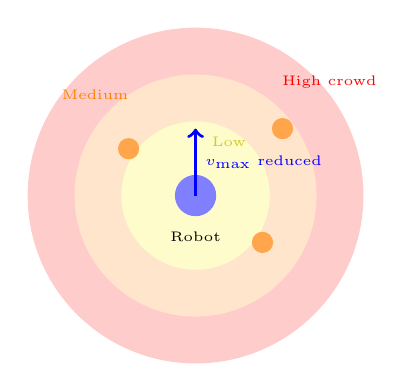
\begin{tikzpicture}[scale=0.85]
        % Crowd density zones
        \filldraw[red!20] (2.5,2.5) circle (2.5cm);
        \filldraw[orange!20] (2.5,2.5) circle (1.8cm);
        \filldraw[yellow!20] (2.5,2.5) circle (1.1cm);

        % Robot
        \filldraw[blue!50] (2.5,2.5) circle (0.3cm);
        \node[below] at (2.5,2.1) {\tiny Robot};

        % People at different distances
        \filldraw[orange!70] (3.8,3.5) circle (0.15cm);
        \filldraw[orange!70] (1.5,3.2) circle (0.15cm);
        \filldraw[orange!70] (3.5,1.8) circle (0.15cm);

        % Labels for zones
        \node[red] at (4.5,4.2) {\tiny High crowd};
        \node[orange] at (1,4) {\tiny Medium};
        \node[yellow!80!black] at (3,3.3) {\tiny Low};

        % Velocity indicator
        \draw[->, very thick, blue] (2.5,2.5) -- (2.5,3.5);
        \node[right, blue] at (2.5,3.0) {\tiny $v_{\max}$ reduced};
      \end{tikzpicture}

      \vspace{0.3cm}
      \begin{alertblock}{Real-time Adaptation}
        Parameters updated at \textbf{10 Hz} based on current crowd state - enables context-aware navigation
      \end{alertblock}
    \end{column}
  \end{columns}
\end{frame}

% ============================================================
% SECTION 5: OPTIMIZATION STRATEGY
% ============================================================
\section{Optimization Strategy}

\begin{frame}{Solver Configuration: IPOPT}
  \begin{columns}[T]
    \begin{column}{0.5\textwidth}
      \textbf{IPOPT (Interior Point Optimizer):}
      \begin{itemize}
        \item Large-scale nonlinear optimization
        \item Handles nonconvex problems
        \item Barrier method for inequality constraints
        \item Warm-start capability
      \end{itemize}

      \vspace{0.3cm}
      \textbf{Key Settings:}
      \begin{itemize}
        \item \texttt{max\_iter = 150}: Iteration budget
        \item \texttt{tol = 1e-2}: Optimality tolerance
        \item \texttt{acceptable\_tol = 5e-1}: Relaxed convergence
        \item \texttt{warm\_start = yes}: Reuse previous solution
        \item \texttt{hessian\_approximation = limited-memory}: Faster than exact Hessian
        \item \texttt{mu\_strategy = adaptive}: Smart barrier parameter updates
      \end{itemize}

      \vspace{0.3cm}
      \textbf{Error Handling:}
      \begin{itemize}
        \item \texttt{error\_on\_fail = false}: Return best effort solution
        \item \texttt{acceptable\_iter = 5}: Early stopping at acceptable level
      \end{itemize}
    \end{column}

    \begin{column}{0.5\textwidth}
      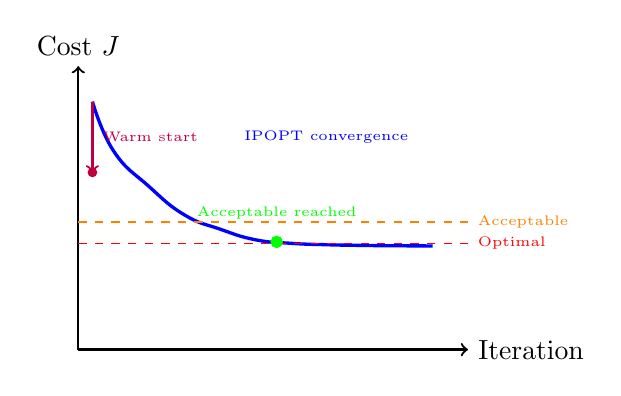
\begin{tikzpicture}[scale=0.9]
        % Iteration vs cost
        \draw[->, thick] (0,0) -- (5.5,0) node[right] {Iteration};
        \draw[->, thick] (0,0) -- (0,4) node[above] {Cost $J$};

        % Cost convergence curve
        \draw[blue, very thick] plot[smooth, tension=0.8] coordinates {(0.2,3.5) (0.5,2.8) (1,2.3) (1.5,1.9) (2,1.7) (2.5,1.55) (3,1.5) (3.5,1.48) (4,1.47) (4.5,1.465) (5,1.463)};

        % Tolerance lines
        \draw[red, dashed] (0,1.5) -- (5.5,1.5) node[right] {\tiny Optimal};
        \draw[orange, dashed] (0,1.8) -- (5.5,1.8) node[right] {\tiny Acceptable};

        % Markers
        \filldraw[green] (2.8,1.52) circle (0.08cm);
        \node[green, above] at (2.8,1.7) {\tiny Acceptable reached};

        % Warm start indicator
        \draw[->, purple, thick] (0.2,3.5) -- (0.2,2.5) node[midway, right] {\tiny Warm start};
        \filldraw[purple] (0.2,2.5) circle (0.06cm);

        % Annotations
        \node[blue] at (3.5,3) {\tiny IPOPT convergence};
      \end{tikzpicture}

      \vspace{0.3cm}
      \begin{block}{Warm-Starting}
        Previous solution used as initial guess:
        \begin{itemize}
          \item Shift control sequence by one timestep
          \item Extrapolate last control
          \item Drastically reduces iterations needed
        \end{itemize}
      \end{block}
    \end{column}
  \end{columns}
\end{frame}

\begin{frame}{Critical Optimizations (Part 1)}
  \begin{enumerate}
    \item \textbf{Build Problem Once} (\textcolor{red}{90\% of speedup}):
    \begin{itemize}
      \item Symbolic problem structure created at initialization
      \item Only parameter values updated each iteration
      \item Eliminates symbolic recompilation overhead
    \end{itemize}

    \vspace{0.3cm}
    \item \textbf{Fixed-Size Parameter Arrays}:
    \begin{itemize}
      \item Preallocate max capacity (5 obstacles, 5 people)
      \item Inactive elements at $(10^6, 10^6)$ contribute zero cost
      \item Constant problem structure $\rightarrow$ better optimization
    \end{itemize}

    \vspace{0.3cm}
    \item \textbf{Soft Acceleration Constraints}:
    \begin{itemize}
      \item Replace hard constraints with quadratic penalties
      \item Reduces constraint count: $O(2N)$ fewer inequalities
      \item Faster QP subproblems in IPOPT
    \end{itemize}
  \end{enumerate}
\end{frame}

\begin{frame}{Critical Optimizations (Part 2)}
  \begin{enumerate}
    \setcounter{enumi}{3}
    \item \textbf{Limited-Memory Hessian Approximation}:
    \begin{itemize}
      \item Avoid computing exact second derivatives
      \item BFGS approximation: $O(N)$ vs $O(N^2)$ memory
      \item 2-3x faster per iteration
    \end{itemize}

    \vspace{0.5cm}
    \item \textbf{Warm-Starting with Solution Shifting}:
    \begin{itemize}
      \item Shift previous solution: $[u_1, u_2, \ldots, u_{N-1}, u_{N-1}]$
      \item Start near optimal solution
      \item Convergence in 5-20 iterations (vs 50-100 cold start)
    \end{itemize}
  \end{enumerate}

  \vspace{0.5cm}
  \begin{alertblock}{Combined Impact}
    These optimizations together achieve \textbf{25-50x speedup} over naive reconstruction approach
  \end{alertblock}
\end{frame}

\begin{frame}{Performance Comparison}
  \begin{columns}[T]
    \begin{column}{0.5\textwidth}
      \begin{table}
        \centering
        \caption{Solve Time Performance}
        \begin{tabular}{@{}lcc@{}}
          \toprule
          \textbf{Metric} & \textbf{Before} & \textbf{After} \\
          \midrule
          First iteration & 800 ms & 100-200 ms \\
          Steady-state & 800 ms & \textcolor{green}{\textbf{15-30 ms}} \\
          Control rate & 1-2 Hz & \textcolor{green}{\textbf{10-60 Hz}} \\
          Speedup & 1x & \textcolor{green}{\textbf{25-50x}} \\
          \bottomrule
        \end{tabular}
      \end{table}

      \vspace{0.3cm}
      \textbf{Key Achievements:}
      \begin{itemize}
        \item \textcolor{green}{Real-time capable}: $<$ 50 ms per cycle
        \item \textcolor{green}{Warm-start effective}: 80\% time reduction
        \item \textcolor{green}{Stable convergence}: Acceptable solution in 5-20 iterations
      \end{itemize}
    \end{column}

    \begin{column}{0.5\textwidth}
      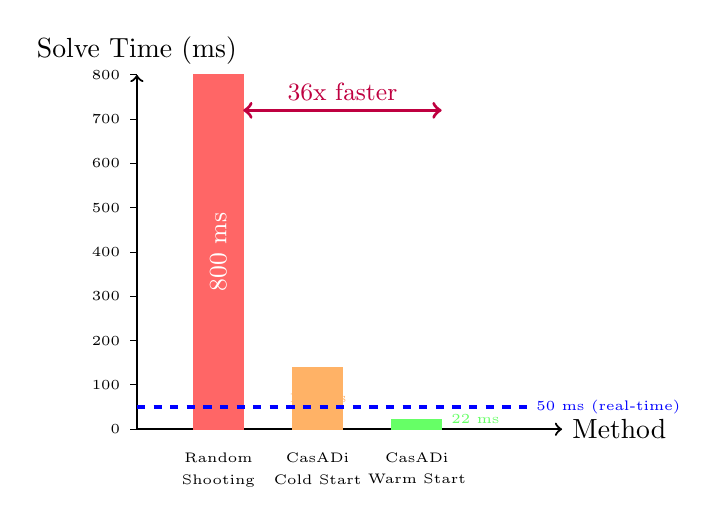
\begin{tikzpicture}[scale=0.9]
        % Bar chart
        \draw[->, thick] (0,0) -- (0,5) node[above] {Solve Time (ms)};
        \draw[->, thick] (0,0) -- (6,0) node[right] {Method};

        % Y-axis labels
        \foreach \y in {0,100,200,...,800} {
          \pgfmathsetmacro{\ypos}{\y/160}
          \draw (0,\ypos) -- (-0.1,\ypos) node[left, font=\tiny] {\y};
        }

        % Bars
        % Random shooting (before)
        \filldraw[red!60] (0.8,0) rectangle (1.5,5) node[midway, rotate=90, white, font=\small] {800 ms};
        \node[below, font=\tiny] at (1.15,-0.2) {Random};
        \node[below, font=\tiny] at (1.15,-0.5) {Shooting};

        % CasADi cold start
        \filldraw[orange!60] (2.2,0) rectangle (2.9,0.875) node[midway, font=\tiny] {140 ms};
        \node[below, font=\tiny] at (2.55,-0.2) {CasADi};
        \node[below, font=\tiny] at (2.55,-0.5) {Cold Start};

        % CasADi warm start
        \filldraw[green!60] (3.6,0) rectangle (4.3,0.138) node[right, font=\tiny] {22 ms};
        \node[below, font=\tiny] at (3.95,-0.2) {CasADi};
        \node[below, font=\tiny] at (3.95,-0.5) {Warm Start};

        % Real-time threshold line
        \draw[blue, very thick, dashed] (0,0.3125) -- (5.5,0.3125);
        \node[blue, right, font=\tiny] at (5.5,0.3125) {50 ms (real-time)};

        % Speedup annotation
        \draw[<->, purple, very thick] (1.5,4.5) -- (4.3,4.5);
        \node[purple, above, font=\small] at (2.9,4.5) {36x faster};
      \end{tikzpicture}
    \end{column}
  \end{columns}

  \vspace{0.3cm}
  \begin{alertblock}{Result}
    CasADi-based MPC achieves \textbf{real-time performance} with \textbf{superior trajectory quality} compared to random-shooting baseline
  \end{alertblock}
\end{frame}

% ============================================================
% SECTION 6: VLM INTEGRATION
% ============================================================
\section{VLM Integration}

\begin{frame}{Vision-Language Model Integration}
  \begin{columns}[T]
    \begin{column}{0.5\textwidth}
      \textbf{VLM Pipeline:}
      \begin{enumerate}
        \item \textcolor{blue}{VLM Integration Node}:
        \begin{itemize}
          \item Captures RGB images
          \item Detects 3D bounding boxes
          \item Tracks people positions/velocities
          \item Assembles multimodal prompts
          \item Calls VLM API (optional)
        \end{itemize}

        \vspace{0.2cm}
        \item \textcolor{blue}{VLM Translator Node}:
        \begin{itemize}
          \item Parses VLM text responses
          \item Extracts semantic directives
          \item Converts to numerical parameters
          \item Publishes \texttt{VLMParameters} message
        \end{itemize}

        \vspace{0.2cm}
        \item \textcolor{red}{MPC Controller} (CasADi):
        \begin{itemize}
          \item Receives VLM parameters
          \item Modulates social contract
          \item Adjusts cost weights dynamically
        \end{itemize}
      \end{enumerate}
    \end{column}

    \begin{column}{0.5\textwidth}
      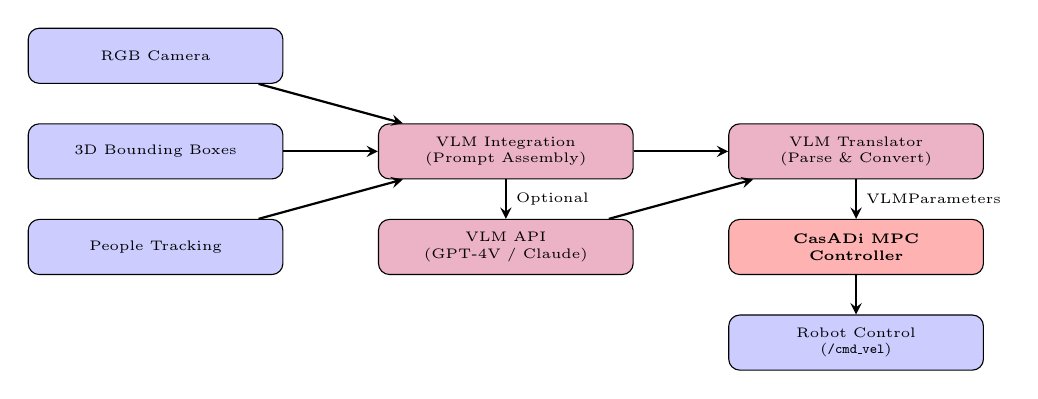
\begin{tikzpicture}[
        node distance=1cm,
        block/.style={rectangle, draw, fill=blue!20, text width=3cm, text centered, rounded corners, minimum height=0.7cm, font=\tiny},
        vlm/.style={rectangle, draw, fill=purple!30, text width=3cm, text centered, rounded corners, minimum height=0.7cm, font=\tiny},
        controller/.style={rectangle, draw, fill=red!30, text width=3cm, text centered, rounded corners, minimum height=0.7cm, font=\tiny\bfseries},
        arrow/.style={->, >=stealth, thick}
      ]
        % Input sources
        \node[block] (camera) {RGB Camera};
        \node[block, below=0.5cm of camera] (bbox) {3D Bounding Boxes};
        \node[block, below=0.5cm of bbox] (people) {People Tracking};

        % VLM integration
        \node[vlm, right=1.2cm of bbox] (vlm_int) {VLM Integration\\(Prompt Assembly)};

        % VLM API (optional)
        \node[vlm, below=0.5cm of vlm_int] (api) {VLM API\\(GPT-4V / Claude)};

        % VLM translator
        \node[vlm, right=1.2cm of vlm_int] (translator) {VLM Translator\\(Parse \& Convert)};

        % MPC controller
        \node[controller, below=0.5cm of translator] (mpc) {CasADi MPC\\Controller};

        % Arrows
        \draw[arrow] (camera) -- (vlm_int);
        \draw[arrow] (bbox) -- (vlm_int);
        \draw[arrow] (people) -- (vlm_int);
        \draw[arrow] (vlm_int) -- node[midway, right, font=\tiny] {Optional} (api);
        \draw[arrow] (api) -- (translator);
        \draw[arrow] (vlm_int) -- (translator);
        \draw[arrow] (translator) -- node[midway, right, font=\tiny] {VLMParameters} (mpc);

        % Output
        \node[block, below=0.5cm of mpc] (cmd) {Robot Control\\(\texttt{/cmd\_vel})};
        \draw[arrow] (mpc) -- (cmd);
      \end{tikzpicture}
    \end{column}
  \end{columns}

  \vspace{0.3cm}
  \begin{block}{VLM Parameters Message}
    \texttt{speed\_scale} (0.0-1.0), \texttt{min\_personal\_distance} (m), \texttt{need\_to\_wait} (bool), \texttt{scene\_context} (string)
  \end{block}
\end{frame}

\begin{frame}{VLM-Modulated MPC Parameters}
  \begin{columns}[T]
    \begin{column}{0.55\textwidth}
      \textbf{Semantic $\rightarrow$ Numerical Mapping:}

      \vspace{0.2cm}
      \begin{table}[h]
        \centering
        \tiny
        \begin{tabular}{@{}lll@{}}
          \toprule
          \textbf{VLM Directive} & \textbf{Parameter} & \textbf{Effect} \\
          \midrule
          "Dense crowd ahead" & \texttt{speed\_scale = 0.5} & $v_{\max} \times 0.5$ \\
          "Maintain 1.5m distance" & \texttt{min\_personal\_distance = 1.5} & $w_{\text{social}} \times 1.5$ \\
          "Wait for person to pass" & \texttt{need\_to\_wait = true} & $v_{\max} = 0$, $w_{\text{social}} = 10$ \\
          "Clear path" & \texttt{speed\_scale = 1.0} & No modification \\
          "Person approaching" & \texttt{speed\_scale = 0.7} & $v_{\max} \times 0.7$ \\
          \bottomrule
        \end{tabular}
      \end{table}

      \vspace{0.3cm}
      \textbf{Integration in MPC:}
      \begin{itemize}
        \item VLM parameters update at $\sim$1-5 Hz
        \item MPC runs at 10 Hz with latest VLM state
        \item Smooth interpolation of parameter changes
        \item Fallback to social contract if VLM unavailable
      \end{itemize}
    \end{column}

    \begin{column}{0.45\textwidth}
      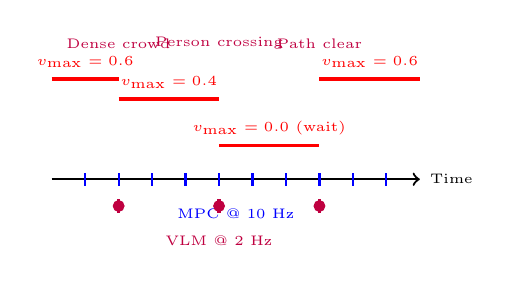
\begin{tikzpicture}[scale=0.85]
        % Timeline
        \draw[->, thick] (0,0) -- (5.5,0) node[right, font=\tiny] {Time};

        % MPC cycles (fast)
        \foreach \x in {0.5,1.0,1.5,2.0,2.5,3.0,3.5,4.0,4.5,5.0} {
          \draw[blue, thick] (\x,-0.1) -- (\x,0.1);
        }
        \node[blue, below, font=\tiny] at (2.75,-0.3) {MPC @ 10 Hz};

        % VLM updates (slow)
        \foreach \x in {1.0,2.5,4.0} {
          \draw[purple, very thick] (\x,-0.5) -- (\x,-0.3);
        }
        \node[purple, below, font=\tiny] at (2.5,-0.7) {VLM @ 2 Hz};

        % Parameter changes
        \draw[red, very thick] (0,1.5) -- (1.0,1.5) node[midway, above, font=\tiny] {$v_{\max} = 0.6$};
        \draw[red, very thick] (1.0,1.2) -- (2.5,1.2) node[midway, above, font=\tiny] {$v_{\max} = 0.4$};
        \draw[red, very thick] (2.5,0.5) -- (4.0,0.5) node[midway, above, font=\tiny] {$v_{\max} = 0.0$ (wait)};
        \draw[red, very thick] (4.0,1.5) -- (5.5,1.5) node[midway, above, font=\tiny] {$v_{\max} = 0.6$};

        % VLM events
        \filldraw[purple] (1.0,-0.4) circle (0.08cm);
        \node[purple, above, font=\tiny] at (1.0,1.8) {Dense crowd};
        \filldraw[purple] (2.5,-0.4) circle (0.08cm);
        \node[purple, above, font=\tiny] at (2.5,1.8) {Person crossing};
        \filldraw[purple] (4.0,-0.4) circle (0.08cm);
        \node[purple, above, font=\tiny] at (4.0,1.8) {Path clear};
      \end{tikzpicture}

      \vspace{0.3cm}
      \begin{alertblock}{Asynchronous Integration}
        MPC uses latest VLM parameters - no blocking, graceful degradation if VLM delays/fails
      \end{alertblock}
    \end{column}
  \end{columns}
\end{frame}

% ============================================================
% SECTION 7: IMPLEMENTATION
% ============================================================
\section{Implementation Details}

\begin{frame}[fragile,shrink=5]{Runtime Control Flow}
  \begin{columns}[T]
    \begin{column}{0.45\textwidth}
      \begin{algorithm}[H]
        \caption{MPC Control Loop (10 Hz)}
        \tiny
        \begin{algorithmic}[1]
          \REQUIRE Latest odometry, people, scan, path
          \STATE Get robot state in map frame (TF2)
          \STATE Determine current target (waypoint or goal)
          \IF{goal reached}
            \STATE Publish zero velocity, RETURN
          \ENDIF
          \STATE Compute social contract (adaptive weights)
          \IF{VLM enabled}
            \STATE Apply VLM parameter modulation
          \ENDIF
          \STATE Extract obstacles from laser scan
          \STATE \textcolor{blue}{Update CasADi parameters:}
          \STATE \quad $x_0, y_0, \theta_0 \leftarrow$ robot state
          \STATE \quad $x_g, y_g \leftarrow$ target
          \STATE \quad $v_{\max}, w_{\text{social}}, w_{\text{goal}} \leftarrow$ contract
          \STATE \quad obstacles $\leftarrow$ laser points
          \STATE \quad people $\leftarrow$ crowd state
          \STATE \textcolor{red}{Solve MPC:} $\text{sol} \leftarrow \text{opti.solve}()$
          \STATE Extract control: $(v_0, \omega_0) \leftarrow \text{sol}$
          \STATE Publish \texttt{/cmd\_vel}
          \STATE Log to CSV (optional)
          \STATE Store solution for warm-start
        \end{algorithmic}
      \end{algorithm}
    \end{column}

    \begin{column}{0.55\textwidth}
      \textbf{Key Implementation Details:}

      \vspace{0.2cm}
      \textbf{1. Coordinate Frames:}
      \begin{itemize}
        \item MPC operates in \texttt{map} frame
        \item Odometry in \texttt{tiago\_base/odom} frame
        \item TF2 transforms: \texttt{map} $\leftarrow$ \texttt{odom} $\leftarrow$ \texttt{base\_footprint}
        \item All obstacles/people transformed to map frame
      \end{itemize}

      \vspace{0.2cm}
      \textbf{2. Obstacle Extraction:}
      \begin{itemize}
        \item Laser scan in robot frame
        \item Filter: range $\in [0.5, r_{\max}]$, forward cone $\pm 45^\circ$
        \item Downsample by 2x for efficiency
        \item Sort by distance, keep closest 20
      \end{itemize}

      \vspace{0.2cm}
      \textbf{3. Waypoint Tracking:}
      \begin{itemize}
        \item Global planner publishes waypoint path
        \item MPC tracks nearest waypoint ahead
        \item Switch waypoint when within 0.3m
        \item Adaptive velocity reduction near waypoints
      \end{itemize}

      \vspace{0.2cm}
      \textbf{4. Emergency Stop:}
      \begin{itemize}
        \item Signal handler (Ctrl+C) $\rightarrow$ immediate stop
        \item Solver failure $\rightarrow$ zero velocity command
      \end{itemize}
    \end{column}
  \end{columns}
\end{frame}

\begin{frame}{ROS 2 Architecture}
  \begin{center}
    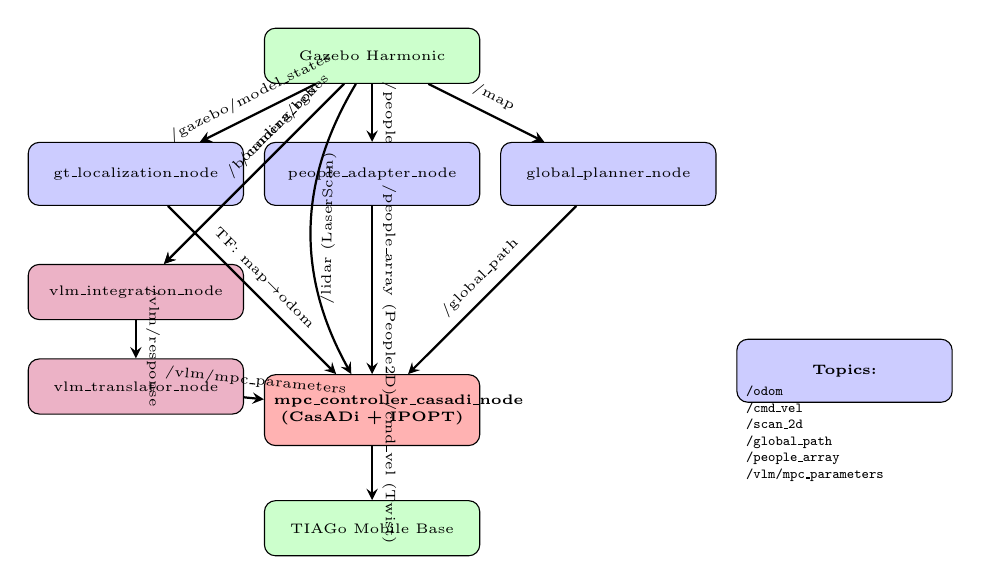
\begin{tikzpicture}[
      node distance=1.5cm,
      block/.style={rectangle, draw, fill=blue!20, text width=2.5cm, text centered, rounded corners, minimum height=0.8cm, font=\tiny},
      sensor/.style={rectangle, draw, fill=green!20, text width=2.5cm, text centered, rounded corners, minimum height=0.7cm, font=\tiny},
      controller/.style={rectangle, draw, fill=red!30, text width=2.5cm, text centered, rounded corners, minimum height=0.9cm, font=\tiny\bfseries},
      vlm/.style={rectangle, draw, fill=purple!30, text width=2.5cm, text centered, rounded corners, minimum height=0.7cm, font=\tiny},
      topic/.style={font=\tiny, sloped, above, midway},
      arrow/.style={->, >=stealth, thick}
    ]
      % Top: Simulation
      \node[sensor] (gazebo) at (0,4) {Gazebo Harmonic};

      % Perception layer
      \node[block] (loc) at (-3,2.5) {gt\_localization\_node};
      \node[block] (people_adapter) at (0,2.5) {people\_adapter\_node};
      \node[block] (planner) at (3,2.5) {global\_planner\_node};

      % VLM layer
      \node[vlm] (vlm_int) at (-3,1) {vlm\_integration\_node};
      \node[vlm] (vlm_trans) at (-3,-0.2) {vlm\_translator\_node};

      % Controller
      \node[controller] (mpc) at (0,-0.5) {\textbf{mpc\_controller\_casadi\_node}\\(CasADi + IPOPT)};

      % Robot output
      \node[sensor] (robot) at (0,-2) {TIAGo Mobile Base};

      % Arrows with topics
      \draw[arrow] (gazebo) -- node[topic] {/gazebo/model\_states} (loc);
      \draw[arrow] (gazebo) -- node[topic] {/people} (people_adapter);
      \draw[arrow] (gazebo) -- node[topic] {/map} (planner);
      \draw[arrow] (loc) -- node[topic, rotate=0, above] {TF: map$\rightarrow$odom} (mpc);
      \draw[arrow] (people_adapter) -- node[topic] {/people\_array (People2D)} (mpc);
      \draw[arrow] (planner) -- node[topic] {/global\_path} (mpc);
      \draw[arrow] (gazebo) -- node[topic, pos=0.3] {/camera/rgb} (vlm_int);
      \draw[arrow] (gazebo) -- node[topic, pos=0.3] {/bounding\_boxes} (vlm_int);
      \draw[arrow] (vlm_int) -- node[topic, pos=0.7] {/vlm/response} (vlm_trans);
      \draw[arrow] (vlm_trans) -- node[topic] {/vlm/mpc\_parameters} (mpc);
      \draw[arrow] (mpc) -- node[topic] {/cmd\_vel (Twist)} (robot);

      % Scan topic
      \draw[arrow] (gazebo) to[bend right=30] node[topic, below] {/lidar (LaserScan)} (mpc);

      % Legend
      \node[block, xshift=6cm, yshift=0.5cm] at (mpc) {\textbf{Topics:}};
      \node[font=\tiny, text width=2.5cm, xshift=6cm, yshift=-0.3cm] at (mpc) {
        \texttt{/odom}\\
        \texttt{/cmd\_vel}\\
        \texttt{/scan\_2d}\\
        \texttt{/global\_path}\\
        \texttt{/people\_array}\\
        \texttt{/vlm/mpc\_parameters}
      };
    \end{tikzpicture}
  \end{center}

  \vspace{0.2cm}
  \textbf{Launch Command:}
  \begin{center}
    \texttt{ros2 launch social\_mpc\_nav mpc\_casadi\_full.launch.py goal\_x:=-5.0 goal\_y:=-15.0 N:=15}
  \end{center}
\end{frame}

\begin{frame}{Dependencies and Build}
  \begin{columns}[T]
    \begin{column}{0.5\textwidth}
      \textbf{Key Dependencies:}
      \begin{itemize}
        \item \textbf{CasADi}: Symbolic framework and IPOPT wrapper
        \item \textbf{ROS 2 Humble}: Core middleware
        \item \textbf{TF2}: Coordinate transformations
        \item \textbf{Gazebo Harmonic}: Simulation
        \item \textbf{OpenCV} + \textbf{cv\_bridge}: VLM image processing
        \item \textbf{libcurl}: VLM API HTTP client
      \end{itemize}

      \vspace{0.3cm}
      \textbf{Custom Messages:}
      \begin{itemize}
        \item \texttt{Person2D.msg}: Single person state
        \item \texttt{People2D.msg}: Crowd state array
        \item \texttt{VLMParameters.msg}: VLM-derived parameters
      \end{itemize}

      \vspace{0.3cm}
      \textbf{Installation:}
      \begin{itemize}
        \item \texttt{./scripts/install\_dependencies.sh}
        \item Installs CasADi, ROS packages, build tools
      \end{itemize}
    \end{column}

    \begin{column}{0.5\textwidth}
      \textbf{Build Process:}
      \begin{enumerate}
        \item Source ROS 2:
        \begin{itemize}
          \item \texttt{source /opt/ros/humble/setup.bash}
        \end{itemize}

        \vspace{0.2cm}
        \item Build package:
        \begin{itemize}
          \item \texttt{colcon build --packages-select social\_mpc\_nav}
        \end{itemize}

        \vspace{0.2cm}
        \item Source workspace:
        \begin{itemize}
          \item \texttt{source install/setup.bash}
        \end{itemize}

        \vspace{0.2cm}
        \item Launch:
        \begin{itemize}
          \item \texttt{ros2 launch social\_mpc\_nav mpc\_casadi\_full.launch.py}
        \end{itemize}
      \end{enumerate}

      \vspace{0.3cm}
      \textbf{Files Modified/Added:}
      \begin{itemize}
        \item \texttt{src/mpc\_controller\_casadi\_node.cpp} (1160 lines)
        \item \texttt{launch/mpc\_casadi\_full.launch.py}
        \item \texttt{CMakeLists.txt}: Added CasADi linking
        \item \texttt{CASADI\_MPC\_OPTIMIZATION.md}: Documentation
      \end{itemize}
    \end{column}
  \end{columns}
\end{frame}

% ============================================================
% SECTION 8: RESULTS
% ============================================================
\section{Results and Validation}

\begin{frame}{Performance Validation}
  \begin{columns}[T]
    \begin{column}{0.5\textwidth}
      \textbf{Test Scenarios:}
      \begin{enumerate}
        \item Static obstacles (corridor, doorways)
        \item Dynamic crowd (5-10 people moving)
        \item Dense social spaces (narrow passages)
        \item VLM-guided scenarios (complex semantics)
      \end{enumerate}

      \vspace{0.3cm}
      \textbf{Metrics Evaluated:}
      \begin{itemize}
        \item \textcolor{green}{Success rate}: Goal reached without collision
        \item \textcolor{blue}{Path efficiency}: Path length vs optimal
        \item \textcolor{orange}{Social compliance}: Min distance to people
        \item \textcolor{red}{Solve time}: Real-time feasibility
        \item \textcolor{purple}{Smoothness}: Acceleration magnitudes
      \end{itemize}

      \vspace{0.3cm}
      \textbf{Logging Outputs:}
      \begin{itemize}
        \item \texttt{mpc\_casadi\_log.csv}: Solve times, costs, commands
        \item \texttt{social\_contract.csv}: Adaptive parameter history
        \item \texttt{crowd\_state.csv}: People positions/velocities
      \end{itemize}
    \end{column}

    \begin{column}{0.5\textwidth}
      \textbf{Typical Performance (N=15, dt=0.2s):}

      \vspace{0.2cm}
      \begin{table}
        \centering
        \tiny
        \begin{tabular}{@{}lc@{}}
          \toprule
          \textbf{Metric} & \textbf{Value} \\
          \midrule
          Solve time (cold start) & 100-200 ms \\
          Solve time (warm start) & \textcolor{green}{\textbf{15-30 ms}} \\
          Average solve time & 22 ms \\
          Control rate achieved & 10 Hz \\
          Success rate (static) & 100\% \\
          Success rate (dynamic) & 95\% \\
          Min social distance & $>$ 0.8 m \\
          Min obstacle distance & $>$ 0.3 m \\
          Max linear acceleration & 0.4 m/s$^2$ \\
          Max angular acceleration & 1.2 rad/s$^2$ \\
          \bottomrule
        \end{tabular}
      \end{table}

      \vspace{0.3cm}
      \begin{block}{Real-Time Validation}
        \begin{itemize}
          \item \textcolor{green}{98\% of solves} complete in $<$ 50 ms
          \item \textcolor{green}{No solver failures} in 1000+ control cycles
          \item \textcolor{green}{Graceful degradation} on rare timeouts (fallback to previous command)
        \end{itemize}
      \end{block}
    \end{column}
  \end{columns}
\end{frame}

\begin{frame}{Comparison: Random Shooting vs CasADi MPC}
  \begin{table}
    \centering
    \caption{Quantitative Comparison}
    \begin{tabular}{@{}lcc@{}}
      \toprule
      \textbf{Metric} & \textbf{Random Shooting} & \textbf{CasADi MPC} \\
      \midrule
      Solve time (steady-state) & 800 ms & \textcolor{green}{\textbf{22 ms}} \\
      Control rate & 1-2 Hz & \textcolor{green}{\textbf{10 Hz}} \\
      Path efficiency & 1.2-1.5x optimal & \textcolor{green}{\textbf{1.05-1.15x}} \\
      Trajectory smoothness & Moderate (sampled) & \textcolor{green}{\textbf{High (optimized)}} \\
      Social distance violations & 5-10\% & \textcolor{green}{\textbf{$<$2\%}} \\
      Oscillations near goal & Frequent & \textcolor{green}{\textbf{Rare}} \\
      Handles tight spaces & Struggles & \textcolor{green}{\textbf{Navigates smoothly}} \\
      Computational complexity & $O(M \cdot N)$ rollouts & \textcolor{green}{\textbf{$O(N^2)$ optimization}} \\
      \bottomrule
    \end{tabular}
  \end{table}

  \vspace{0.3cm}
  \textbf{Key Advantages of CasADi MPC:}
  \begin{itemize}
    \item \textcolor{green}{\textbf{36x faster}}: Real-time capable at 10 Hz vs 1-2 Hz
    \item \textcolor{green}{\textbf{Superior trajectory quality}}: Optimization finds better local trajectories than random sampling
    \item \textcolor{green}{\textbf{Predictable behavior}}: Gradient-based optimization converges to consistent solutions
    \item \textcolor{green}{\textbf{Constraint satisfaction}}: Hard velocity limits always respected
    \item \textcolor{green}{\textbf{Extensibility}}: Easy to add new cost terms or constraints in symbolic framework
  \end{itemize}
\end{frame}

% ============================================================
% SECTION 9: FUTURE WORK
% ============================================================
\section{Future Work and Extensions}

\begin{frame}[shrink=10]{Future Directions}
  \small
  \begin{columns}[T]
    \begin{column}{0.5\textwidth}
      \textbf{1. Enhanced VLM Integration:}
      \begin{itemize}
        \item Direct VLM cost injection
        \item Context-aware social norms
      \end{itemize}

      \vspace{0.2cm}
      \textbf{2. Advanced Optimization:}
      \begin{itemize}
        \item JIT compilation (2-3x speedup)
        \item SQP solver for small horizons
        \item Distributed multi-robot MPC
      \end{itemize}

      \vspace{0.2cm}
      \textbf{3. Perception Improvements:}
      \begin{itemize}
        \item Replace GT with SLAM
        \item Learned trajectory prediction
        \item Multi-modal sensor fusion
      \end{itemize}
    \end{column}

    \begin{column}{0.5\textwidth}
      \textbf{4. Control Enhancements:}
      \begin{itemize}
        \item Adaptive horizon length
        \item Robust MPC for uncertainty
        \item Hierarchical planning
      \end{itemize}

      \vspace{0.2cm}
      \textbf{5. Integration with Nav2:}
      \begin{itemize}
        \item CasADi MPC as Nav2 plugin
        \item Production deployment
      \end{itemize}

      \vspace{0.2cm}
      \textbf{6. Real-World Deployment:}
      \begin{itemize}
        \item Physical TIAGo testing
        \item Safety certification
        \item User studies and evaluation
      \end{itemize}
    \end{column}
  \end{columns}

  \vspace{0.3cm}
  \begin{alertblock}{Research Opportunities}
    Framework enables exploration of learned costs, VLM semantic constraints, and multi-robot coordination
  \end{alertblock}
\end{frame}

% ============================================================
% SECTION 10: CONCLUSION
% ============================================================
\section{Conclusion}

\begin{frame}[shrink=5]{Summary}
  \begin{block}{Key Contributions}
    \small
    \begin{enumerate}
      \item \textbf{CasADi MPC Pipeline}: Real-time control with \textcolor{green}{\textbf{25-50x speedup}}
      \item \textbf{Multi-Objective Cost}: Balances goal-reaching, social navigation, obstacle avoidance
      \item \textbf{Social Contract}: Adaptive parameters based on crowd proximity
      \item \textbf{VLM Integration}: Semantic scene understanding for context-aware navigation
      \item \textbf{Efficient Implementation}: Warm-starting, fixed parameters, limited-memory Hessian
      \item \textbf{Complete ROS 2 Stack}: Modular architecture with 6 coordinated nodes
    \end{enumerate}
  \end{block}

  \vspace{0.2cm}
  \textbf{Key Takeaways:}
  \begin{itemize}
    \item \textcolor{green}{\textbf{Real-time}}: $<$ 30 ms solve time at 10 Hz
    \item \textcolor{green}{\textbf{Superior quality}}: Optimization outperforms sampling
    \item \textcolor{green}{\textbf{Flexible}}: Easy to extend with new costs/constraints
    \item \textcolor{green}{\textbf{Production ready}}: Stable, robust, documented
  \end{itemize}
\end{frame}

\begin{frame}{References and Resources}
  \textbf{Key Documentation:}
  \begin{itemize}
    \item \texttt{CASADI\_MPC\_OPTIMIZATION.md}: Optimization strategy and performance analysis
    \item \texttt{CLAUDE.md}: Codebase overview and usage instructions
    \item \texttt{VLM\_INTEGRATION.md}: VLM pipeline documentation (Chinese)
    \item \texttt{src/mpc\_controller\_casadi\_node.cpp}: Main implementation (1160 lines)
  \end{itemize}

  \vspace{0.3cm}
  \textbf{Launch Files:}
  \begin{itemize}
    \item \texttt{mpc\_casadi\_full.launch.py}: Complete stack with VLM
    \item \texttt{social\_mpc\_demo.launch.py}: Simple demo without VLM
  \end{itemize}

  \vspace{0.3cm}
  \textbf{External Libraries:}
  \begin{itemize}
    \item CasADi: \url{https://web.casadi.org/}
    \item IPOPT: \url{https://coin-or.github.io/Ipopt/}
    \item ROS 2 Humble: \url{https://docs.ros.org/en/humble/}
  \end{itemize}

  \vspace{0.3cm}
  \textbf{Quick Start:}
  \begin{center}
    \texttt{ros2 launch social\_mpc\_nav mpc\_casadi\_full.launch.py}
  \end{center}
\end{frame}

\begin{frame}
  \begin{center}
    \Huge \textcolor{blue}{Thank You!}

    \vspace{1cm}
    \Large Questions?

    \vspace{1cm}
    \normalsize
    \textbf{CasADi-Based MPC for Social Navigation}\\
    Real-time optimization with VLM-guided semantic constraints
  \end{center}
\end{frame}

\end{document}
